% !TEX root = poster.tex
\node [mybox,anchor=north west, font=\fontsize{\fntszL}{\fntszL}\selectfont]
at (\goalPos) (boxGoal){%
\begin{minipage}{\bxszA}

 \bigskip
 \bigskip
 \bigskip

 \textbf{
 \centerline{
 Develop statistical framework for model error
 }
 \centerline{
representation, quantification and propagation
}
\centerline{
\underline{for physical models.}
 }
 }

  \vspace*{-1cm}

 \begin{itemize}
 \item Represent and estimate the error associated with
 \begin{itemize}
\item Simplifying assumptions, parameterizations
\item Mathematical formulation, theoretical framework
\item Numerical discretization
\end{itemize}
%\vspace*{-1.4cm}
%\item Inverse modeling context $\qquad\overbrace{y_i}^{\textrm{Data}} = \overbrace{f(x_i;\lambda)}^{\textrm{Model}} + \overbrace{\epsilon_i}^{\textrm{Meas. error}}$
\vspace*{-0.2cm}
\item Inverse modeling context $\qquad y_i =f(x_i;\lambda) +\epsilon_i$
\item Given data, calibrate for $\lambda$, accounting for model error
\medskip
\item Model error is deviation from `truth'
\end{itemize}

\medskip
\medskip
\medskip

\centerline{
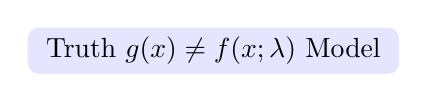
\begin{tikzpicture} \node [rounded corners,fill=blue!10] {
$\textrm{ Truth } g(x) \neq f(x;\lambda) \textrm{ Model }$
};
\end{tikzpicture}
}

\medskip
\medskip
\medskip
% \textbf{\centerline{Represent and estimate the error associated with}}
% \medskip
% \textbf{...will be useful for }
% \begin{itemize}
% \item Model validation
% \item Model comparison
% \item Scientific discovery and model improvement
% \item Reliable computational predictions
% \end{itemize}


\end{minipage}
};
\node[fancytitle, right=10pt, font=\fontsize{\fntszL}{\fntszL}\selectfont]
at (boxGoal.north west) {\bf Goal: Model Error Quantification};
